% Report
\documentclass{article}

% Here set the various packages
% Packages to load
\usepackage[english]{babel}
% %%% Support some german text
% \usepackage{ngerman}
% \usepackage[latin1]{inputenc}   % für Umlaute
%%%
% \usepackage[utf8]{inputenc}
\usepackage[T1]{fontenc}
\usepackage{microtype}

%%%
% \usepackage[inline]{enumitem} % Required for the "description" list.

%%% Fix for not hyperlinking citations
\makeatletter
\let\NAT@parse\undefined
\makeatother
\usepackage{hyperref}
% 
\usepackage{cite}
% \ifx\pdfoutput\undefined
% 	\usepackage{graphicx}
% \else
% 	\usepackage[pdftex]{graphicx}
% \fi
\usepackage{graphicx}
\graphicspath{{Figures/}}
\usepackage{amsmath}
% \interdisplaylinepenalty=2500

% Shading of questions. Use the "shaded" environment or the "\hl{}" command.
\usepackage{framed}
% \usepackage[dvipsnames]{color}
\usepackage[svgnames]{xcolor}
\usepackage{soul}
% Nice colours: Gainsboro, LightGoldenrod, LightSteelBlue
% furter ref: https://www.latextemplates.com/svgnames-colors
\definecolor{shadecolor}{named}{Gainsboro}
\sethlcolor{Gainsboro}

%%% Todo margin notes (enable/disable)
\usepackage{todonotes}
% \usepackage[disable]{todonotes}
%%%

%eof

%%%

\title{Programming of Supercomputers\\Worksheet 3}
\author{
	\begin{tabular}{rl}
		Oleksandr Voloshyn& \texttt{<o.voloshyn@tum.de>}\\ 
		Qunsheng Huang& \texttt{<keefe.huang@tum.de>}\\ 
		Tommaso Bianucci& \texttt{<bianucci@in.tum.de>}
	\end{tabular}
}
\date{\today}

\begin{document}

\maketitle
\renewcommand{\abstractname}{Group members's contributions}
\begin{abstract}
	\begin{center}
		\begin{tabular}{rl}
		% Here write the contributions of the members of the group
		Oleksandr Voloshyn:& worked on 1, 3\\
		Qunsheng Huang:& worked on 1, 3\\
		Tommaso Bianucci:& worked on 2
		\end{tabular}
	\end{center}
\end{abstract}

\section{Setting a Baseline}
\subsection{Required submission files}
\begin{enumerate}
	\item \hl{The updated Load-Leveler batch script.}

		\verb!Data/Baseline/updated_job.ll!

	\item \hl{The performance plots and description in the report.}

		Figures \ref{fig:IO}, \ref{fig:setup}, \ref{fig:total}, \ref{fig:varying_size}, and\ref{fig:varying_domain} show the various performance plots for the baseline. A Vampir baseline plot is shown in Fig. \ref{fig:vampir_baseline}.

\end{enumerate}

\subsection{Questions}
\begin{enumerate}
	\item \hl{Briefly describe the Gaussian Elimination and the provided implementation.}

	The Gaussian Elimination (GE) is a program that converts a dense matrix into an upper-right triangular matrix. A naive implementation is as follows:
\begin{enumerate}
	\item Choosing a pivot. This is typically the value in the diagonal. In the current implementation, no shifting of rows is done and this ignored for the naive implementation.
	\item The factor $\frac{a_{ij}}{a_{ii}}$ is calculated for each row in the column that is below the diagonal, such that $i > j$ if the topmost leftmost matrix entry is set as $a_{00}$.
	\item The pivot row, multiplied by the calculated factor, is subtracted from each row below the pivot row. This sets the column below the pivot to zero.
\end{enumerate}

The provided implementation implements a few changes to simplify the calculations done in parallel.

Firstly, the full matrix is read in by process 0. The root process then performs some ordering of the matrix data and sends rows of the matrix to each process. Asserts are put in place to ensure that:
\begin{itemize}
	\item The number of rows are equal to the number of columns
	\item The number of processes must fully divide the number of rows/columns.
\end{itemize}

The algorithm then works as follows:
\begin{enumerate}
\item Determine pivot entry: Each loop in the GE algorithm sets all values in a column below the diagonal to zero via linear operations. This is a purely sequential task, there is always only one pivot entry at one point in time and the current pivot is always on the diagonal entry of the current worked row. We refer to the process in charge of updating the rows containing the current pivot entry as the \textit{current process}. 

An assert is put in place to ensure that this pivot value not zero. 
\item Normalize rows: all values in the row, including the RHS value, is first normalized by the pivot entry 
\begin{equation*}
	a_{ij}^{(norm)} = \frac{a_{ij}}{a_{ii}} \quad \forall j \in [1, \# Cols]
\end{equation*}
and 
\begin{equation*}
rhs_{i}^{(norm)} = \frac{rhs_{i}}{a_{ii}} \quad \forall i \in [1, \# Rows].
\end{equation*}

\item Perform elimation step in current process: All values directly below the current pivot entry are set to zero by subtracting the pivot row multiplied by $a_{ki}$. Since the pivot entry is always set to 1, the linear operation reduces each non-zero element in the given rows $k$ per:
\begin{equation*}
	a_{kj} \,-=\, a_{ij}^{(norm)} \cdot a_{ki} \quad \,i < j < \# Cols, \, i < k < \# Rows,
\end{equation*}
where i is the row of the current pivot entry. The pivot then shifts to the diagonal entry in the next row and the process is repeated until the current process has looped through all rows it controls.
\item Communication of normalized values: All normalized values in the matrix and the rhs are stored in given buffers and sent to each process with a higher rank than the current process. 
\item Perform elimination step on processes that are not the current process.
\item Change current process: The pivot then shifts to a row governed by a new process and the normalization, elimination and communication steps are repeated until all processes are complete. Note that the process with rank $size-1$ does not communicate the normalized values.
\item Aggregate solution data to process 0: Backward elimination is performed so that the effect of all non-zero elements not on the diagonal is removed. As the diagonal entries are all now 1, this becomes the identity matrix and the solution vector $x$ is equal to the rhs vector $b$. All processes send solution data to proces 0.
\end{enumerate}

Effectively, information is sent to each processor in a sequential, cascading manner fowards. The Gaussian Elimination (GE) code presents a major challenge in load-balancing---as the algorithm progresses, the amount of work available for each process decreases. When the last few rows are undergoing GE, all but one process is still performing work. 

We ran vampir on the baseline process to observe the blocking \verb!MPI_Send! and \verb!MPI_Recv! functions. This can be seen in Fig. \ref{fig:vampir_baseline}.

 \begin{figure}[h] % h=here, t=top, b=bottom, p=(extra)page, !=force
 	\begin{center}
  		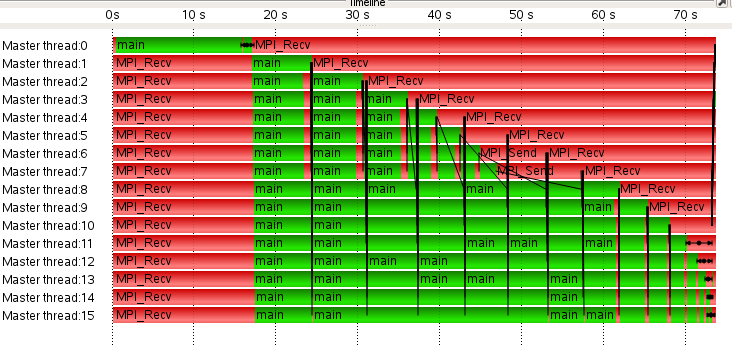
\includegraphics[width=.7\linewidth]{Baseline/vampir_baseline.png} % It searches in the Figures/ folder!
  		\caption{Vampir Benchmark}
  		\label{fig:vampir_baseline}
  	\end{center}
 \end{figure}

	\item \hl{How is data distributed among the processes?}

	Each process takes a number of rows of the matrix equal to $\frac{row}{\#processes}$. There are checks in place such that the number of processes must be able to fully divide the total number of rows.

	\item \hl{Explain the changes applied to the provided Load-Leveler batch script.}

	One of the main difficulties is getting a good average value for the times. As such, the main way to reduce variance in results is to run each instance multiple times. In our case, we ran the code 5 times for each combination of MPI processes and domain size.

	\vspace{5mm} % This is to push next item to next page
	\item \hl{What were the challenges in getting an accurate baseline time for Gaussian Elimination.}

	The main challenges were to determine what was important when determining a baseline. When improving the aglorithm, the main focus will be to reduce the amount of sequential communication---so that each process is able to receive updated information with as little wait time as possible. Thus, our chosen baseline should show improvement when the communication algorithm is improved. The following show the respective baselines chosen for each of the measured times:
\begin{enumerate}
	\item I/O Time

	I/O is only performed on the main process or process 0. Thus, it only makes sense to note this from process 0. Fig. shows the average time for I/O operations in process 0 for the various domain sizes. Since the I/O operation takes place completely sequentially, the number of processes does not affect the times. We see the average I/O times for each domain size in the Fig. \ref{fig:IO}.
	
	
% % Figure example
 \begin{figure}[h] % h=here, t=top, b=bottom, p=(extra)page, !=force
 	\begin{center}
  		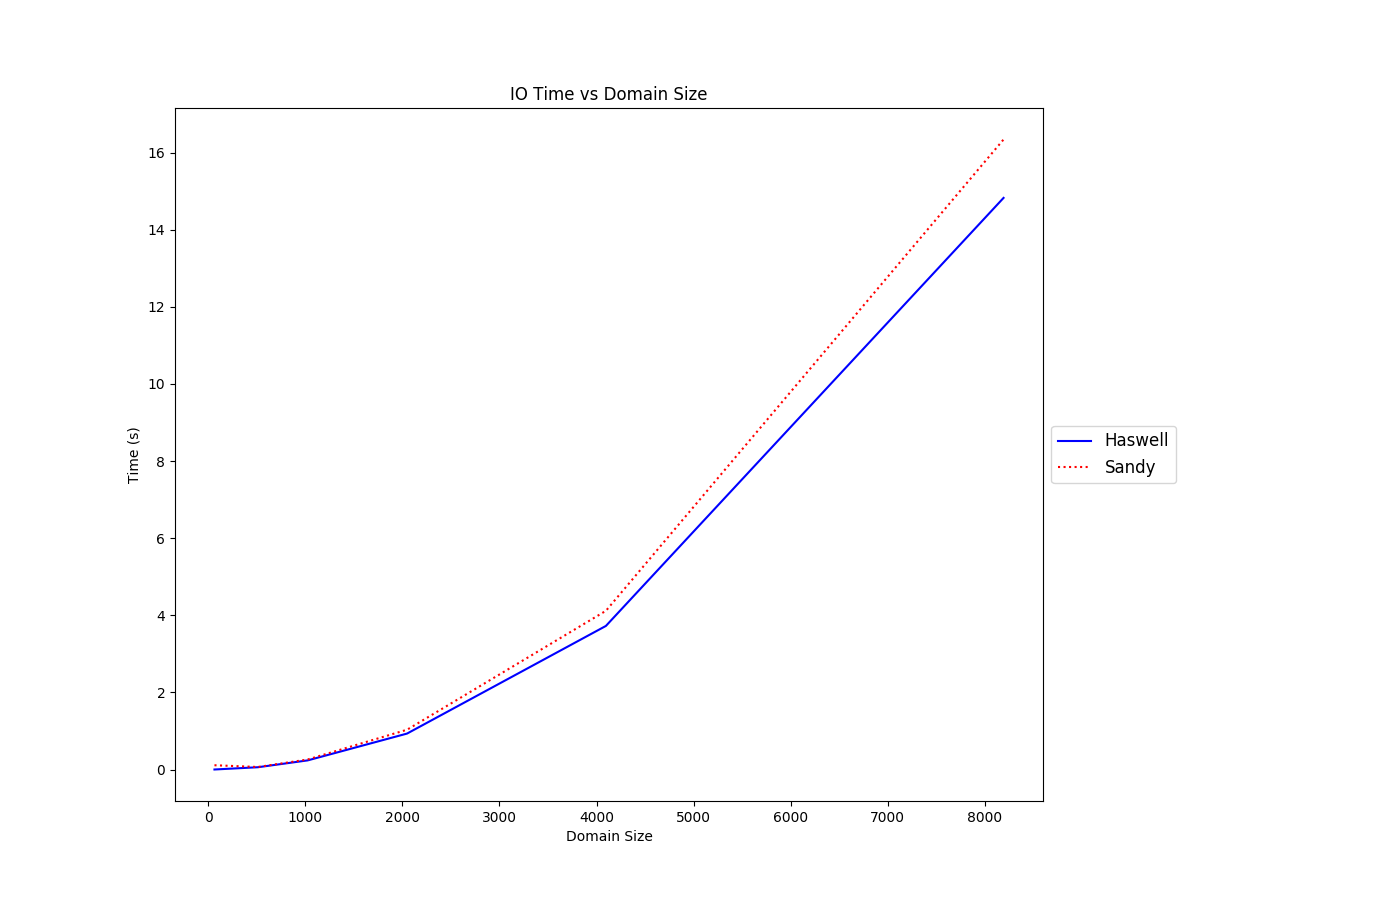
\includegraphics[width=.7\linewidth]{Baseline/io_baseline.png} % It searches in the Figures/ folder!
  		\caption{I/O Time vs. Domain Size}
  		\label{fig:IO}
  	\end{center}
 \end{figure}

	\item Setup Time

	The setup time measures the amount of time each process waits before they fully receive their local matrix rows and local rows of the RHS vector. Since the sending process from process 0 is sequential, process 0 uses blocking communication to send data to process 1, 2, 3 ... etc, some processes with higher rank will wait for a longer time. Fig. \ref{fig:setup} shows the \textit{longest} wait time of all processes. 
	
	We see that keeping the domain size constant and increasing the number of processes, shown in Fig. \ref{fig:setup}(a), results in relatively constant setup times. This only changes for the smaller domain sizes of 1024, 512 and 64 with a larger number of processes. This likely is due to the communication overhead beginning to dominate.
	
 We also see that the setup time increases with the total domain size---which make sense as a larger domain necesitates more data sent from the root process to each other process. This can be seen for any number of processes, as shown in Fig. \ref{fig:setup}(b). Additionally, we see again the poor performance for smaller domain sizes with a high number of processes.
	
	
	\begin{figure}[h] % h=here, t=top, b=bottom, p=(extra)page, !=force
		\begin{tabular}{cc}
			\hspace*{-0.35\linewidth}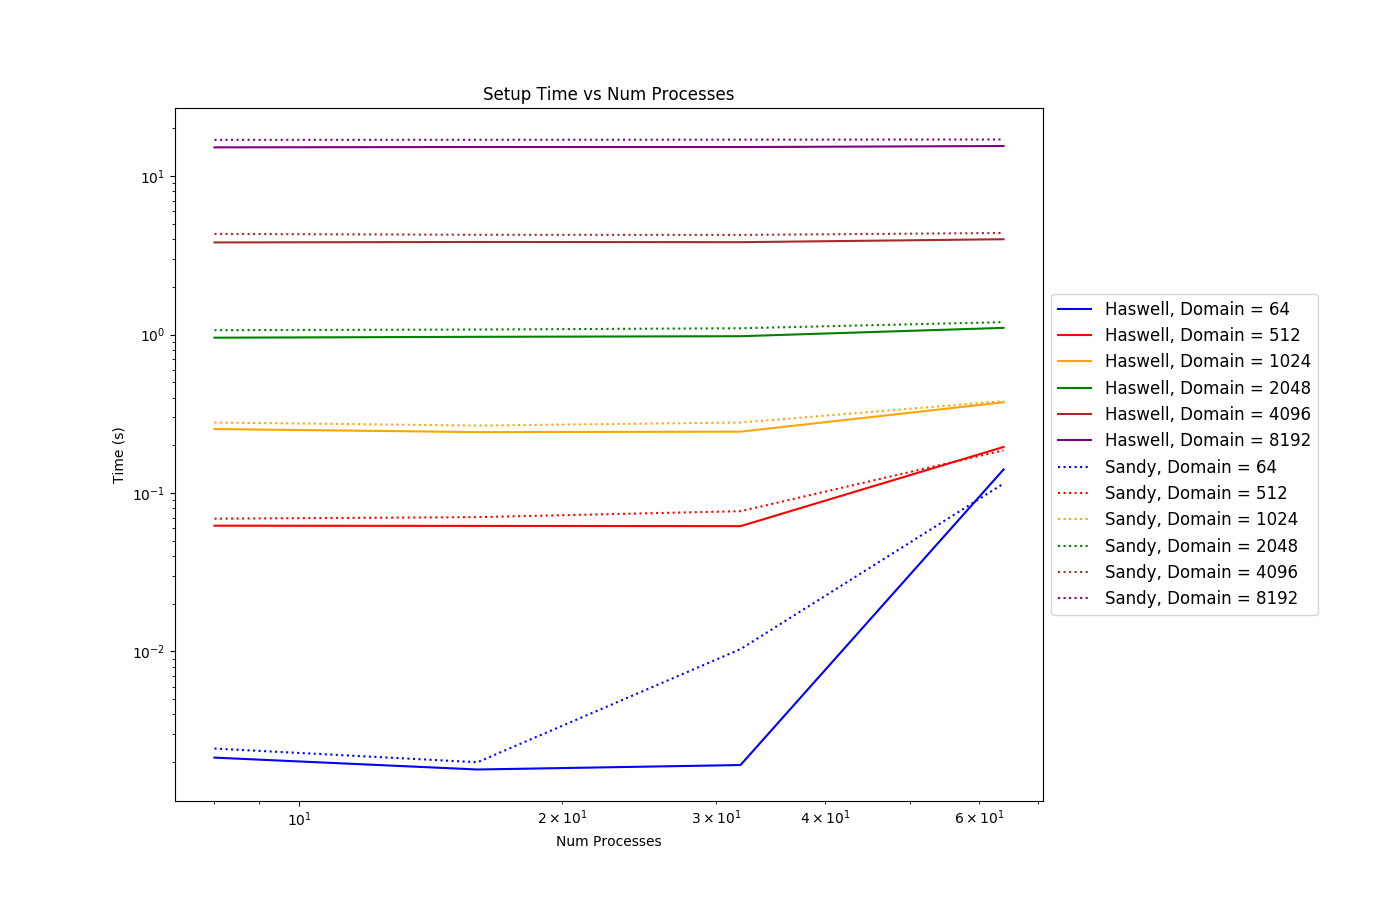
\includegraphics[width=.85\linewidth]{Baseline/setup_multdomain_baseline.png} & \hspace*{-0.05\linewidth}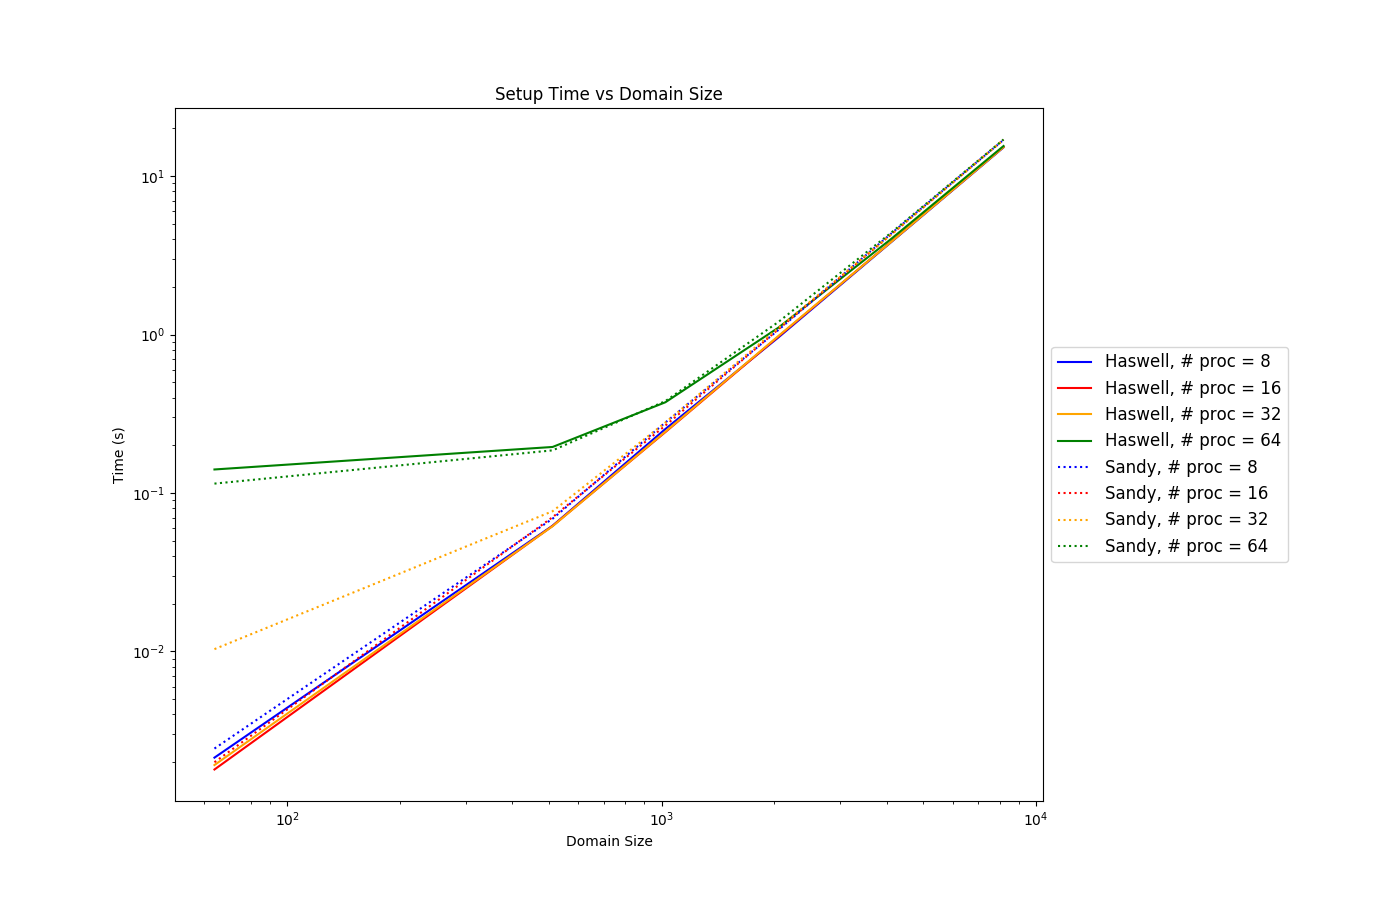
\includegraphics[width=.85\linewidth]{Baseline/setup_multproc_baseline.png} \\
		    \hspace*{-0.45\linewidth}(a) Fixed Domain Size Varying \#Processes & \hspace*{-0.15\linewidth}(b) Fixed \#Processes Varying Domain Size\\[6pt]\\
		\end{tabular}
		\caption{Setup Time, Haswell vs. Sandy Bridge.}
		\label{fig:setup}
	\end{figure}
	
	\item Compute Time
	
	The compute time measures the amount of time between the start of the gaussian elimination steps to the end of the gaussian elimination steps. This includes the MPI time. Therefore, to determine the actual compute time, we subtract the MPI time from the compute time and average the results across the multiple processes. This is because the overall computational work for each domain size should remain relatively constant---regardless of the number of processes used. If an algorithmic improvement occurs in the code, this should improve this benchmark.
	
	\item MPI Time
	
	The MPI time sums up the total amount of time spent during communication. We hope to decrease this value by improving the communication and computation overlap. The MPI time increases with increased domain size as well and generally decreases with an increased number of nodes (as the amount sent to each node decreases). However, for very small domain sizes, we see the cost of communication overtake the benefits of multiple nodes. This is seen for domain sizes of 64x64 with 64 processes.
	
	\item Total Time
	
	The total time indicates the amount of time required to fully execute the GE algorithm. We see in Fig. \ref{fig:total}(a), total time generally decreases with an increased number of processes (if the domain size is sufficiently large that communication costs do not outweight the benefits of additional processes performing computation). However, the more interesting plot is Fig. \ref{fig:total}(b), where we can identify the "ideal" number of processes for best performance by tracing the line with the lowest time at each domain size. It is in this graph that we can see when it becomes beneficial to introduce more processes for performing the GE.
 	
 	
 	\begin{figure}[h] % h=here, t=top, b=bottom, p=(extra)page, !=force
		\begin{tabular}{cc}
			\hspace*{-0.35\linewidth}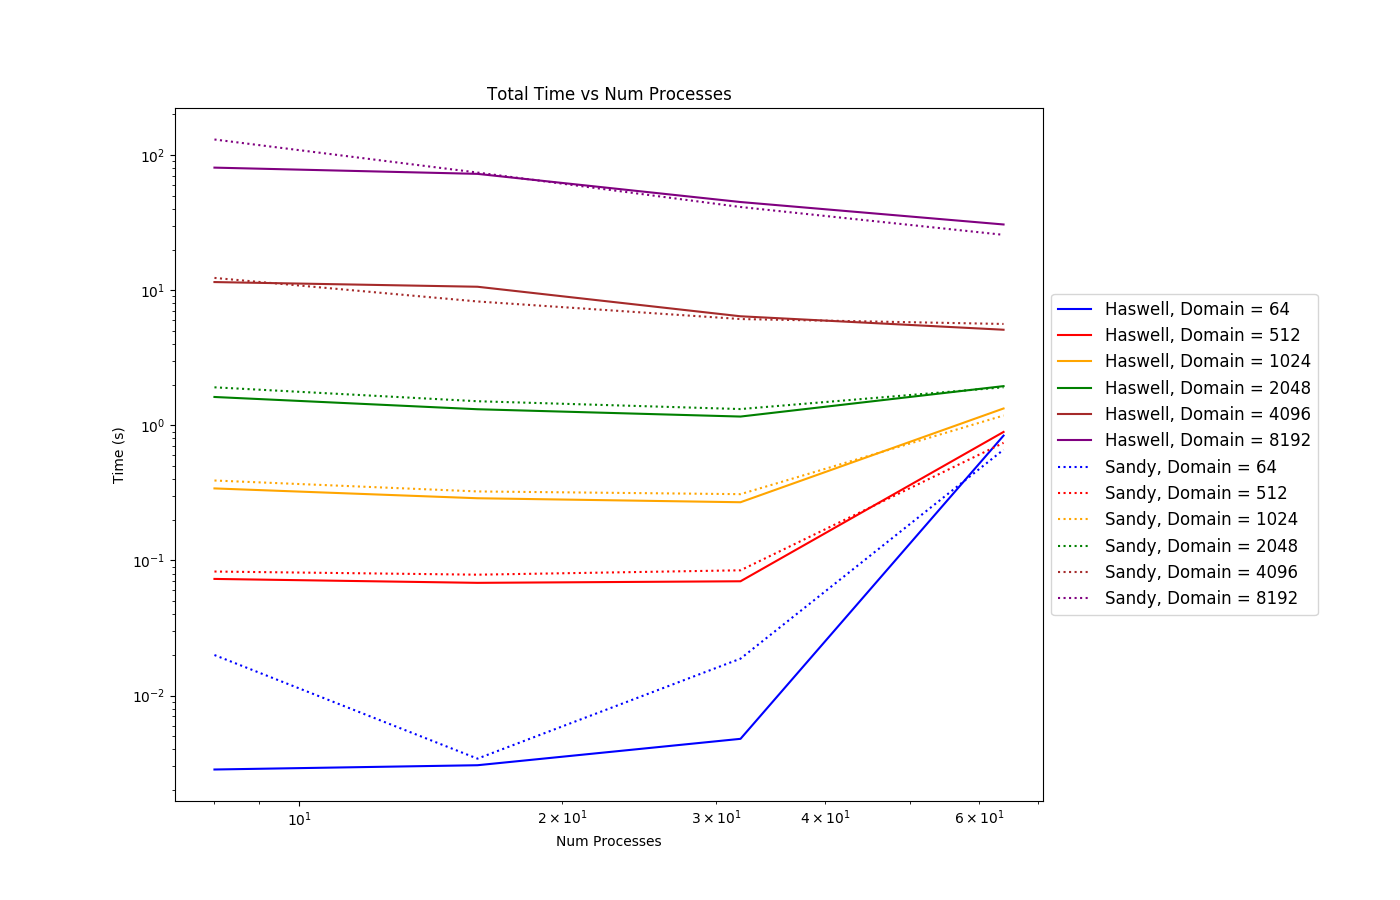
\includegraphics[width=.85\linewidth]{Baseline/total_multdomain_baseline.png} & \hspace*{-0.05\linewidth}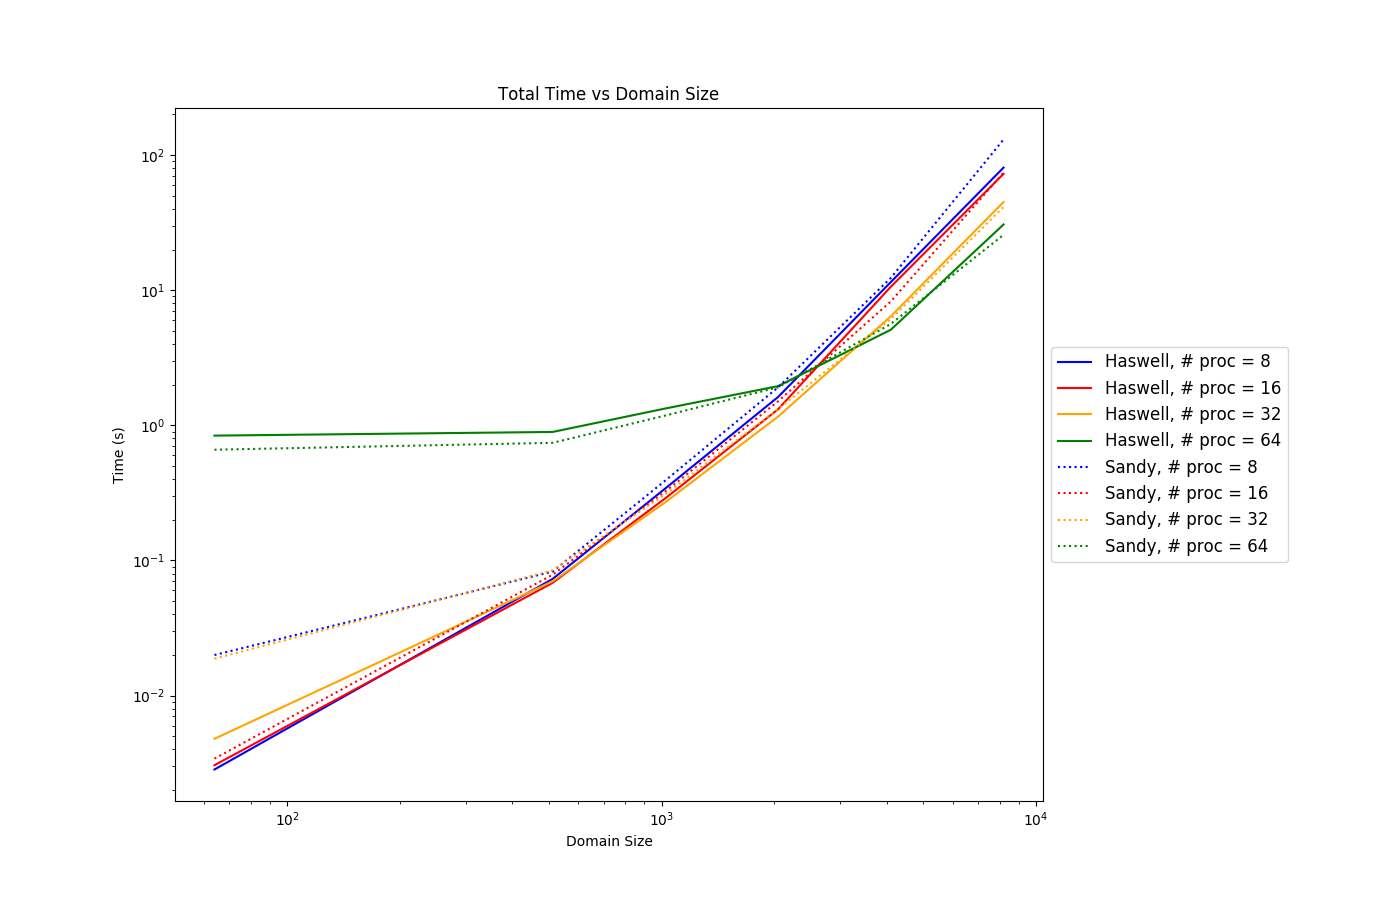
\includegraphics[width=.85\linewidth]{Baseline/total_multproc_baseline.png} \\
		    \hspace*{-0.45\linewidth}(a) Fixed Domain Size Varying \#Processes & \hspace*{-0.15\linewidth}(b) Fixed \#Processes Varying Domain Size\\[6pt]\\
		\end{tabular}
		\caption{Total Time, Haswell vs. Sandy Bridge.}
		\label{fig:total}
	\end{figure}
	\end{enumerate}

	\item \hl{Describe the compute and MPI times scalability with fixed process counts and varying size of input files for the Sandy Bridge and Haswell nodes. Did you observe any differences?}
	
	
	\begin{figure}[h] % h=here, t=top, b=bottom, p=(extra)page, !=force
		\begin{tabular}{cc}
			\hspace*{-0.35\linewidth}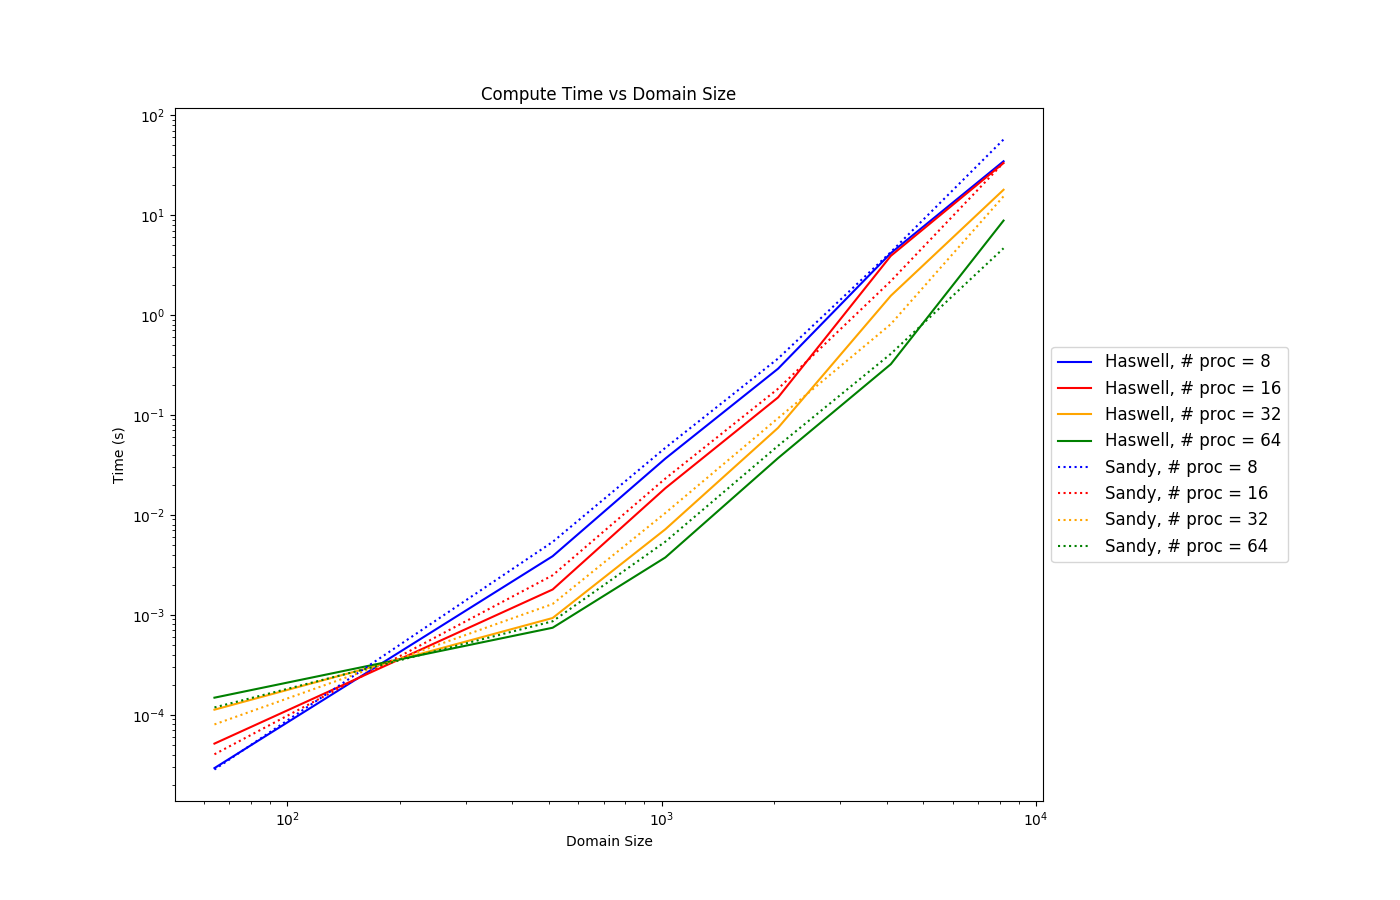
\includegraphics[width=.85\linewidth]{Baseline/compute_multproc_baseline.png} & \hspace*{-0.05\linewidth}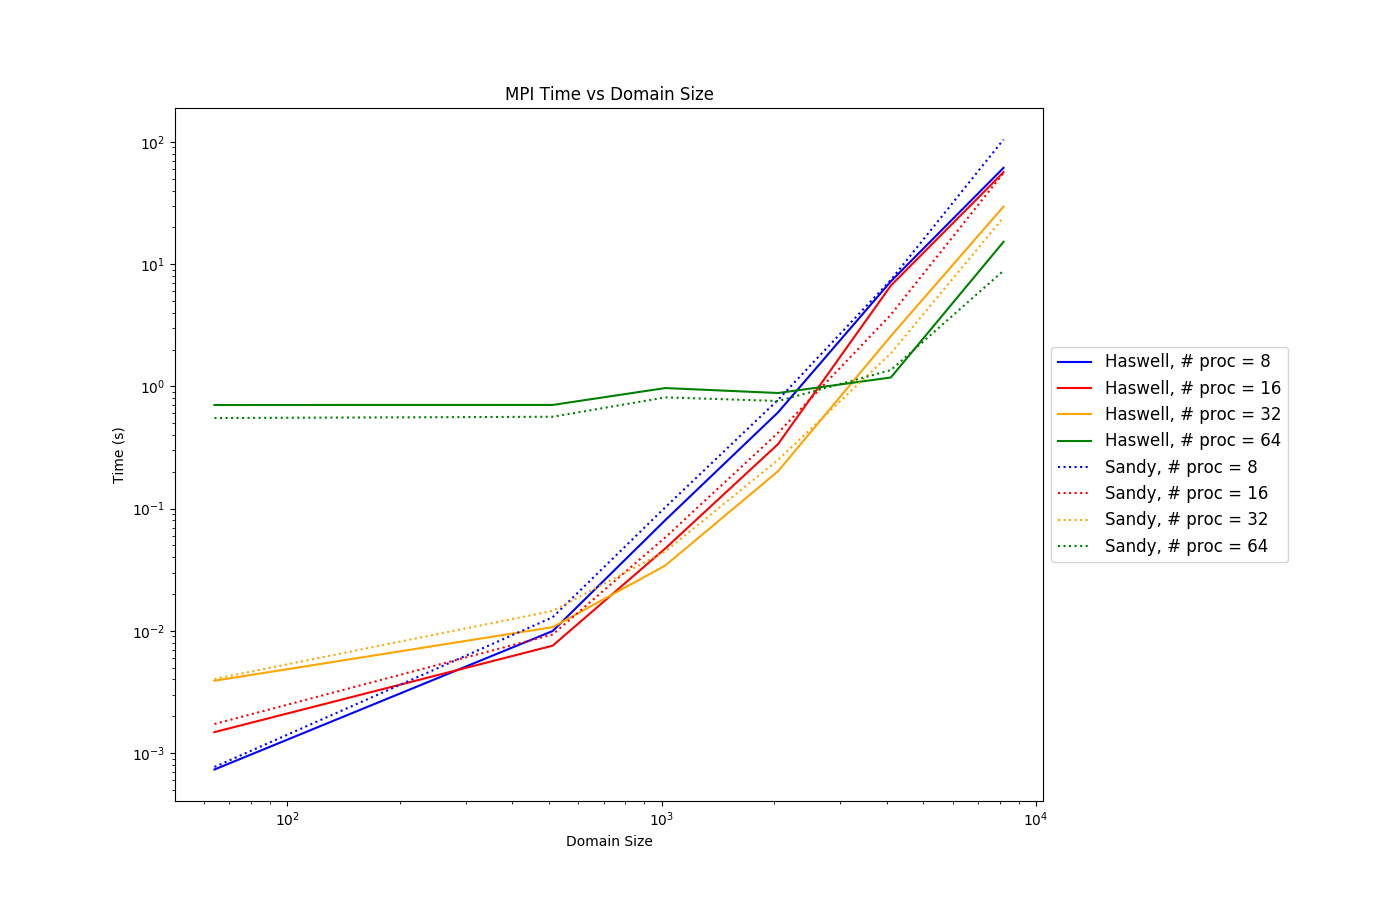
\includegraphics[width=.85\linewidth]{Baseline/mpi_multproc_baseline.png} \\
		    \hspace*{-0.45\linewidth}(a) Compute Time vs. Domain Size & \hspace*{-0.15\linewidth}(b) MPI Time vs. Domain Size\\[6pt]\\
		\end{tabular}
		\caption{Fixed Process Counts \& Varying Size.}
		\label{fig:varying_size}
	\end{figure}
	
	With fixed process count and a varying domain size, we see that the compute time increases with domain size, as shown in Fig \ref{fig:varying_size}(a). This trend was observed in Fig.\ref{fig:total}(b) and is not surprising. When comparing the performance of the Haswell and Sandy Bridge architectures, we see that Haswell nodes perform better for a majority of the time. Haswell nodes generally have shorter compute times when compared with Sandy Bridge when the domain size is between 512 and 4096. However, the Sandy Bridge nodes have shorted compute times at small domain sizes or very large domain sizes with a high number of processes.

	With a fixed domain size and a varying process count, we see, unsurprisingly, in Fig. \ref{fig:varying_size}(b) that the MPI times increase with domain size as more values need to be communicated across processes. We also see that Haswell nodes have shorter MPI times compared to Sandy Bridge nodes for process counts of 8, 16 \& 32 when the domain size is below 4096. When the domain size is increased beyond 4096, Sandy Bridge nodes have shorter MPI times for all process counts other than 8. Additionally, we note that the Sandy Bridge nodes have shorter MPI times for almost any domain size when the process count is increased to 64.
	
	Overall, this seems to indicate that, within these constraints, the Haswell nodes will perform slightly better. However, these results also imply that the Sandy Bridge nodes may scale better with a larger domain size and an increased process count (assuming that the chosen process count is suitable for the given domain size). 

	% \vspace{10mm} % This is to push next item to next page
	\item \hl{Describe the compute and MPI times scalability with fixed input sets and varying process counts for the Sandy Bridge and Haswell nodes. Did you observe any differences?}

	\begin{figure}[h] % h=here, t=top, b=bottom, p=(extra)page, !=force
		\begin{tabular}{cc}
			\hspace*{-0.35\linewidth}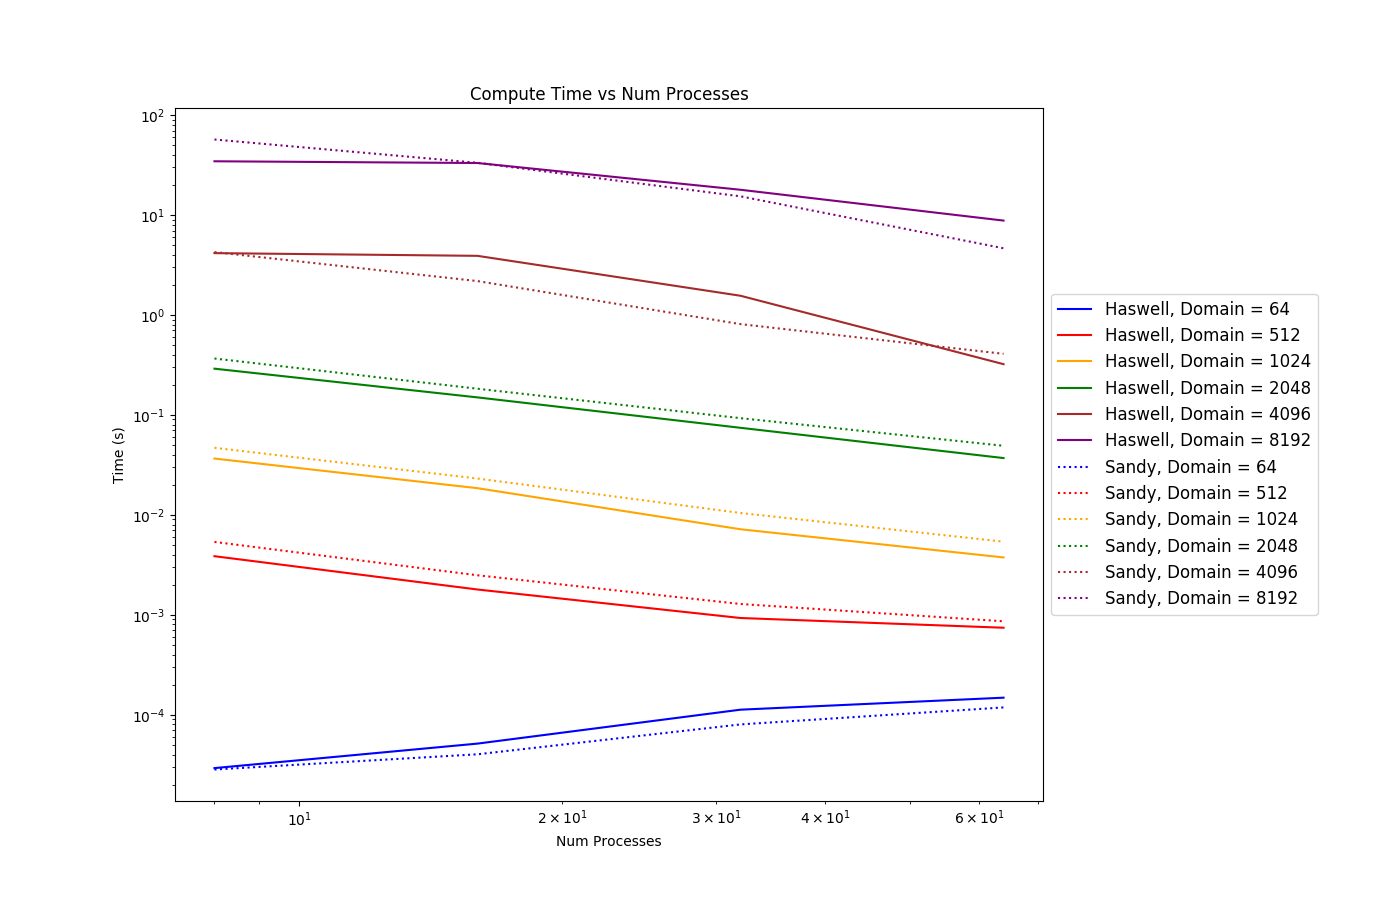
\includegraphics[width=.85\linewidth]{Baseline/compute_multdomain_baseline.png} & \hspace*{-0.05\linewidth}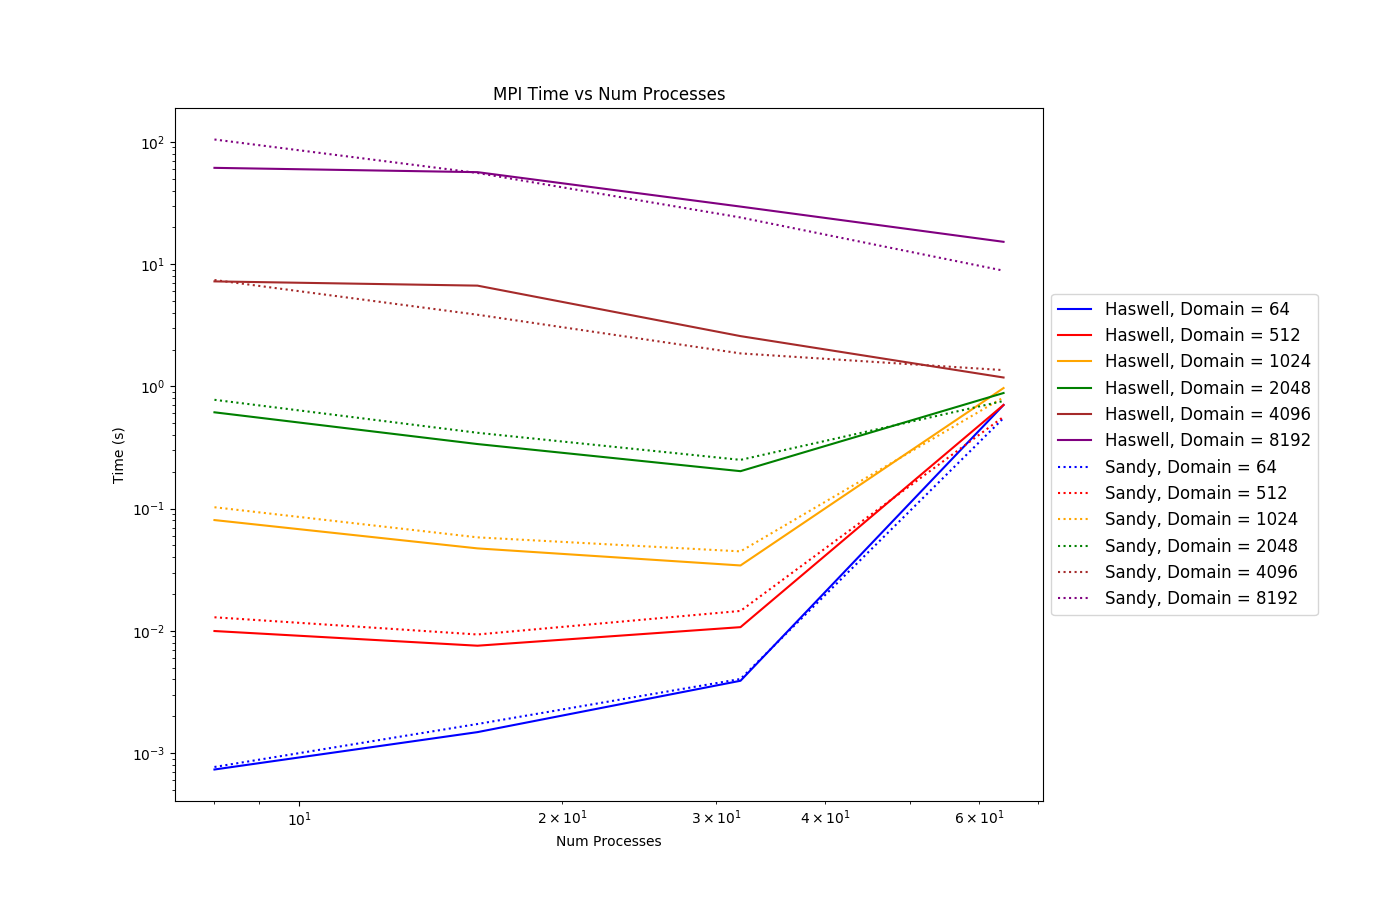
\includegraphics[width=.85\linewidth]{Baseline/mpi_multdomain_baseline.png} \\
			\hspace*{-0.45\linewidth}(a) Compute Time vs. \#Processors & \hspace*{-0.15\linewidth}(b) MPI Time vs. \#Processors\\[6pt]
		\end{tabular}
		\caption{Fixed Size \& Varying Process Counts.}
		\label{fig:varying_domain}
	\end{figure}


With fixed domain size and increasing the process count, we see that the compute time decreases with process count. This is not surprising because each process works on a smaller segment of the full matrix. We see in Fig.\ref{fig:varying_domain} that this remains true for any domain size. For small domain sizes, such as 64x64, the compute time is completely negligible in comparison to the communication time. For larger domain sizes, the compute time becomes much more significant. We see that the Haswell nodes has generally shorter compute times for any processor count. However, the Sandy Bridge nodes still seem to scale better with a larger number of processes at a large domain size.

We expect to see a longer MPI time as the number of processes increase. However, this does not seem to be the case across the board. This is true for the smaller domain sizes, but not the larger domain sizes, as seen in Fig \ref{fig:varying_domain}. This is somewhat surprising as we would expect the cost of comnunication to increase with increased processes. We attribute this observed effect to the sequential nature of the MPI passing---the first process waits for all other processes to finish computing before it returns. As a result, if we successfully overlap compute time with MPI time, we will see a decrease in the time spent waiting for blocking MPI calls.

We see that the Haswell architecture performs better overall, with the Sandy Bridge nodes performing slightly better, with regards to MPI time, for large domains with larger process counts.
\end{enumerate}

% % Figure example
% \begin{figure}[p] % h=here, t=top, b=bottom, p=(extra)page, !=force
%  	\begin{center}
%  		
\includegraphics[width=.9\linewidth]{figure.png} % It searches in the Figures/ folder!
%  		\caption{Caption text}
%  		\label{fig:figureLabelName}
%  	\end{center}
% \end{figure}

\subsection{Questions}
\begin{enumerate}
\item Briefly describe the Gaussian Elimination and the provided implementation.

The Gaussian Elimination (GE) is a program that converts a dense matrix into an upper-right triangular matrix. This is done via a recursive algorithm that sets entire columns of the matrix to zero by:
\begin{enumerate}
\item Choosing a pivot. This is typically the value in the diagonal. Pivoting may be performed to shift the row with the largest value in that column into the correct position
\item The factor $\frac{a_{ij}}{a_{ii}}$ is calculated for each row in the column that is below the diagonal, such that $i > j$ if the topmost leftmost matrix entry is set as $a_{00}$.
\item All rows in the column below the diagonal are set to zero using the calculated factor
\end{enumerate}

The provided implementation uses segments the matrix into rows and provides a set of rows to each process. The value of pivots are sent to each processor in a sequential, cascading manner. Each row then calculates the factor mentioned in the algorithm and then performs the linear operations to set the correct column values to 0.

Gaussian Elmination code presents a major challenge in load-balancing---as the algorithm progresses, the amount of work available for each process decreases. When the last few rows are undergoing GE, all but one process is still performing work. 

\item How is data distributed among the processes?

Each process takes a number of rows of the matrix equal to $\frac{row}/{#processes}$. There are checks in place such that the number of processes must be able to fully divide the total number of rows.

\item Explain the changes applied to the provided Load-Leveler batch script.

One of the main difficulties is getting a good average value for the times. As such, the main way to reduce variance in results is to run each instance multiple times. In our case, we ran the code 5 times for each combination of MPI processes and domain size.

\item What were the challenges in getting an accurate baseline time for Gaussian Elimination.

The main challenges were to determine what was important when determining a baseline. The Gaussian When improving the aglorithm, the main focus will be to reduce the amount of sequential communication---so that each process is able to receive updated information with as little wait time as possible. Thus, our chosen baseline should show improvement when the communication algorithm is improved. The following show the respective baselines chosen for each of the measured times:
\begin{enumerate}
	\item I/O Time

	I/O is only performed on the main process or process 0. Thus, it only makes sense to note this from process 0. Fig. shows the average time for IO operations in process 0 for the various domain sizes. Since the IO operation takes place completely sequentially, the number of processes does not affect the times. 

	\item Setup Time

	The setup time measures the amount of time each process waits before they fully receive their local matrix rows and local rows of the RHS vector. Since the sending process from process 0 is sequential---process 0 uses blocking communication to send data to process 1, 2, 3 ... etc, some processes with higher rank will wait for longer. Improvement will then be indicated by the \textit{longest} wait time of all processes. The provided data shows either the longest wait time for each process
	
	\item Compute Time
	
	The compute time measures the amount of time between the start of the gaussian elimination steps to the end of the gaussian elimination steps. This includes the MPI time. Therefore, to determine the actual compute time, we subtract the MPI time from the compute time. The compute time is extremely small for low values of the domain but grows significantly for larger domains. The compute time always decreases with increasing number of processes.
	
	\time MPI Time
	
	The MPI time sums up the total amount of time spent during communication. We hope to decrease this value by improving the communication and computation overlap. The MPI time increases with increased domain size as well and generally decreases with an increased number of nodes (as the amount sent to each node decreases). However, for very small domain sizes, we see the cost of communication overtake the benefits of multiple nodes. This is seen for domain sizes of 64x64 with 64 processes.
	

	\end{enumerate}


\item Describe the compute and MPI times scalability with fixed process counts and varying size of input
files for the Sandy Bridge and Haswell nodes. Did you observe any differences?

With fixed process count and increasing the domain size, we see that the compute time increases with domain size. This is not surprising as there is more time required for computation. We see in Fig. that this remains true for any number of processes. However, we see that while the Haswell nodes are faster at a 8 processes, the Sandy Bridge nodes are faster when the number of nodes is increased to 64. This seems to indicate that Sandy Bridge processors scale better with a larger number of processes.

We see that the MPI times follow a similar pattern---with a larger domain size, the amount of time in communication increases. This remains true at any number of processes. The shape of the graphs are very similar to that seen for the compute time. We also see similar behavior that the Sandy Bridge processors scale better with a larger number of processes.
 
\item Describe the compute and MPI times scalability with fixed input sets and varying process counts for
the Sandy Bridge and Haswell nodes. Did you observe any differences?

With fixed domain size and increasing the process count, we see that the compute time decreases with process count. This is not surprising because each process works on a smaller segment of the full matrix. We see in Fig. that this remains true for any domain size. For small domain sizes, such as 64x64, the compute time is completely negligible in comparison to the communication time. For larger domain sizes, the compute time becomes much more significant. We see that the Haswell nodes remain faster for any processor when the domain size is small. Once the domain size exceeds a certain threshold, the Sandy Bridge nodes are seen to scale better with a larger number of processes.

We see that the MPI times follow a similar pattern---with more processors, MPI time decreases. This is somewhat surprising as we would expect the cost of comnunication to increase with increased processes. We attribute this observed effect to the sequential nature of the MPI passing---the first process waits for all other processes to finish computing before it returns. As a result, by reducing overall computational time, we decrease the time spent waiting for blocking MPI calls. We see that the Sandy Bridge architecture performs better overall---at very small process counts it is, overall, slightly faster than the Haswell architecture. At larger domain sizes, the difference in MPI times very large, but shrinks with an increasing number of processors.

\end{enumerate}

\section{MPI Point-to-Point Communication}
\subsection{Required submission files}
\begin{enumerate}
	\item \hl{The updated \emph{gauss.c} file.}

		\verb!Data/path/to/file!

	\item \hl{The new performance plots and description in the report.}

		References to figures here...

\end{enumerate}

\subsection{Questions}
\begin{enumerate}
	\item \hl{Which non-blocking operations were used? Justify your choice.}

	Answer...

	\item \hl{Was communication and computation overlap achieved? Use Vampir.}

	Answer...

	\item \hl{Was a speedup observed versus the baseline for the Sandy Bridge and Haswell nodes?}

	Answer...

\end{enumerate}

% % Figure example
% \begin{figure}[p] % h=here, t=top, b=bottom, p=(extra)page, !=force
%  	\begin{center}
%  		
\includegraphics[width=.9\linewidth]{figure.png} % It searches in the Figures/ folder!
%  		\caption{Caption text}
%  		\label{fig:figureLabelName}
%  	\end{center}
% \end{figure}

\section{MPI One-Sided Communication}
\subsection{Required submission files}
\begin{enumerate}
	\item \hl{The updated \emph{gauss.c} file.}

		\verb!Data/path/to/file!

	\item \hl{The new performance plots and description in the report.}

		References to figures here...

\end{enumerate}

\subsection{Questions}
\begin{enumerate}
	\item \hl{Question}

	Answer...

	\item \hl{Question}

	Answer...

	
\end{enumerate}
% % Figure example
% \begin{figure}[p] % h=here, t=top, b=bottom, p=(extra)page, !=force
%  	\begin{center}
%  		
\includegraphics[width=.9\linewidth]{figure.png} % It searches in the Figures/ folder!
%  		\caption{Caption text}
%  		\label{fig:figureLabelName}
%  	\end{center}
% \end{figure}


\end{document}

%eof
